\documentclass[runningheads]{llncs}
\usepackage{amsmath}
\usepackage{booktabs}
\usepackage{color}
\usepackage{graphicx}
\usepackage{hyperref}

\renewcommand\UrlFont{\color{blue}\rmfamily}

\begin{document}

\title{
    Making History Count
}
\author{Gabriele Cerizza}
\authorrunning{G. Cerizza}

\institute{Università degli Studi di Milano\\
\email{gabriele.cerizza@studenti.unimi.it}\\
\url{https://github.com/gabrielecerizza/information_retrieval_project}}

\maketitle

\section{Introduction}
\label{sec:introduction}

In this report we detail our findings in the study of two tasks related to project number 9 for the Information Retrieval course of University of Milan\footnote{\url{https://island.ricerca.di.unimi.it/\~alfio/shared/inforet/2020-21/inforet-projects.html}}: detection of shifts in the meaning of words across time (Section \ref{sec:semantic_shifts}) and extraction of historical events from text (Section \ref{sec:historical_events}).

\section{Semantic shifts}
\label{sec:semantic_shifts}

The first task is concerned with measuring, in a data-driven way, the diachronic semantic shift or lexical semantic change (LSC) that affected words across time. Formally, given a set of words $W$ and two time periods $t_1$ and $t_2$, we want to measure
\begin{equation}
    D(w_{t_1}, w_{t_2}) = \text{distance}(w_{t_1}, w_{t_2}) \,,
\end{equation}
where $w_{t_1}$ and $w_{t_2}$ correspond to the same word $w$ used in corpora of time periods $t_1$ and $t_2$.

We proceed to review known approaches to tackle the problem and then we discuss three possible strategies to measure LSC by exploiting word embeddings originated from a corpus of historical documents and from a corpus of contemporary documents.

\subsection{Related work}
\label{subsec:semantic_shifts:related_work}

In literature, the attempts to capture semantic shifts by way of word embeddings can be categorized in mainly two families: static embeddings or type-based models, and contextualized embeddings or token-based models.

\subsubsection{Static embeddings models} Static embeddings represent each word with a single vector. This vector can be considered a summarization of the occurrences of a word in different contexts. Popular static embeddings are obtained from skip-gram with negative sampling (SGNS)~\cite{mikolov-etal-2013-word2vec}, GloVe~\cite{pennington-etal-2014-glove} and fastText~\cite{bojanowski-etal-2017-fasttext}.

Static embeddings can be exploited to detect semantic shifts in a straightforward way. We train two models on corpora of different time periods and then we measure the cosine distance between the embeddings of a given word obtained from the two models~\cite{hamilton-etal-2016-diachronic}. The issue in this direct comparison is that SGNS and the other neural models are stochastic in nature and therefore they produce embeddings that may be differently rotated along the axes (invariance under rotation). Common solutions include:

\begin{itemize}
    \item orthogonal Procrustes method, which aligns the embeddings to the same coordinate axes~\cite{hamilton-etal-2016-diachronic}, but may introduce noise in the projections~\cite{dubossarsky-etal-2019-time};
    \item initialization of the weights of one model with the weights of the other model, which can be problematic for new words~\cite{kutuzov-etal-2018-diachronic,tahmasebi-etal-2018-survey};
    \item second-order similarity, which first computes the similarity of a word to other words in one vector space, then computes the similarity of the same word to other words in the other vector space, and finally compares the two similarities~\cite{kutuzov-etal-2018-diachronic,tahmasebi-etal-2018-survey}.   
\end{itemize}

\subsubsection{Contextualized embeddings models} Recently developed neural models like BERT~\cite{devlin-etal-2018-bert} generate different word embeddings for each different context in which a word appears. The pretrained contextualized embeddings are sometimes employed by the authors as is, without fine-tuning on the historical corpus~\cite{rother-etal-2020-cmce,laicher-etal-2021-explaining}. 

Contextualized embeddings models start by extracting a vector for each context in which a word appears. A context is  usually a sentence (or a portion thereof) in the two corpora. Then, these models cluster the vectors of the two periods to find the different senses of a word. After that, they measure how the frequency of the senses changed between the time periods to get an estimate of the semantic shift~\cite{giulianelli-etal-2020-analysing,rother-etal-2020-cmce}. An alternative approach computes the average pairwise distance between each vector of one period and each vector of the other period~\cite{laicher-etal-2021-explaining}.  
 

\subsection{Proposed methods}
\label{subsec:semantic_shifts:methods}

We explored three methods to detect semantic shifts. Two are based on static embeddings and a third one on contextualized embeddings.

\subsubsection{Orthogonal Procrustes method (OP)} We started by collecting pretrained static word embeddings. For the historical corpus we used the embeddings provided in~\cite{sprugnoli-tonelli-2019-histo}. These embeddings were trained with fastText on documents dating from 1860 to 1939 and taken from the Corpus of Historical American English (COHA\footnote{\url{https://corpus.byu.edu/coha/}}) for a total of 198M tokens. For the contemporary corpus we used fastText word embeddings trained on Wikipedia and news\footnote{\url{https://fasttext.cc/docs/en/english-vectors.html}} for a total of 16B tokens and 1M word vectors.

Considering the size of the contemporary vocabulary, as well as the fact that it contained misspelled words, we decided to analyze only the 5000 most frequent words in the contemporary vocabulary, intersected with the historical vocabulary. We also made sure to analyze the “target" words indicated by SemEval-2020~\cite{schlechtweg-etal-2020-semeval} for evaluation purposes (see Subsection~\ref{subsec:semantic_shifts:results}).

Finally, we aligned the vectors with orthogonal Procrustes and computed the cosine distance between the two embeddings of each selected word.

\subsubsection{Nearest neighbors method (NN)} This approach leverages ideas taken from the second-order similarity techniques used with static embeddings. We used the same historical and contemporary word embeddings described for OP. Likewise, we analyzed the same words selected for OP.

The proposed second-order similarity is computed as follows. For each selected word we take the 15 nearest neighbors in the historical vector space; then we measure the cosine distance between the word and these neighbors in the historical vector space; after that, we measure the cosine distance between the word and the same neighbors, but this time in the contemporary vector space; finally we compute the mean squared error (MSE) between the distances measured in the historical vector space and the distances measured in the contemporary vector space. Then we do the same for the 15 nearest neighbors in the contemporary model. Finally, we take the mean between the MSE measured on the historical vector space neighbors and the MSE measured on the contemporary vector space neighbors. 

Given this second-order similarity, we decided to shrink the vocabulary of the two models to their intersection. In this way we guaranteed that each neighbor found in one vector space was also present in the other vector space. 

\subsubsection{Jensen-Shannon distance method (JSD)} This method is based on contextualized embeddings. The corpora were taken from SemEval-2020~\cite{schlechtweg-etal-2020-semeval}. The historical corpus contained shuffled sentences from 1810-1860, while the contemporary corpus contained shuffled sentences from 1960-2010. Both corpora were composed of 6M tokens.

We analyzed the 5000 most frequent words in both corpora, keeping only adjectives, nouns and verbs and filtering stop words, punctuations and tokens containing non-alphabetic characters. We aggregated the embeddings according to lemma and POS tags. Our assumption is that the semantic shift of a word is invariant to declension and conjugation: “cat" and “cats" should be subject to the same semantic shift; likewise for “write" and “wrote". Note that in the previous methods we were not able to distinguish words based on POS, since we only had the embeddings, thus the noun “attack" and the verb “attack" had the same embeddings.

We generated the embeddings from BERT, using the “bert-base-cased"\footnote{\url{https://huggingface.co/bert-base-cased}} pretrained weights, by feeding the transformer with sentences from the corpora. We fine-tuned the model on the historical corpus for 5 epochs. Note that we used only one model to generate embeddings for both time periods. Since BERT generates different embeddings for different contexts, it suffices that BERT acquired knowledge of the contexts used in both time periods~\cite{martinc-etal-2020-leveraging}. For the embeddings, we took only the hidden state of the last layer, which is reportedly the layer most related to semantics~\cite{laicher-etal-2021-explaining}.

Following the approach described in~\cite{rother-etal-2020-cmce}, we first employed an autoencoder to reduce the dimensionality of the embeddings from 768 to 20. Then, the dimensionality was further reduced to 10 with UMAP. The combination of autoencoder and UMAP was shown to be effective for clustering in~\cite{mcconville-etal-2019-n2d}. We clustered the embeddings of a given word with HDBSCAN, which is a variant of DBSCAN with improved robustness and a single hyperparameter~\cite{campello-etal-2013-hdbscan}. 

Interpreting the clusters as senses of a word, we measured the frequency of each sense in the two time periods. Finally, we used the Jensen-Shannon distance to measure the similarity between the two distributions.

\subsection{Results}
\label{subsec:semantic_shifts:results}

In Table~\ref{tab:semantic_shifts:top_words} we show the 10 words whose semantic shift was most prominent according to the proposed methods. In OP we can see many words whose meaning changed due to technological evolution, like “cd", “tv" and “bot". OP and NN also capture shifts of historical or cultural nature, like “isis" and “gay". We observe that the International System of Units was introduced in 1960, hence a possible explanation for the shift in “km". The semantic shifts detected by JSD are not as readily decipherable. 

In Figure~\ref{fig:semantic_shifts:score} we give an example of how the shift in senses was perceived by the JSD method. We can see, for instance, that the verb “score" assumed a meaning more related to sports as the time passed.

\begin{table}
    \caption{Top 10 words with the most semantic shift detected by the methods.}
    \label{tab:semantic_shifts:top_words}
    \centering
    \begin{tabular}{lll}
        \toprule
        OP & NN & JSD \\
        \midrule
        cd & deletion & negro (adj.) \\
        romney & km & people (noun) \\
        km & gay & golf (noun) \\
        diff & diff & shopping (noun)  \\
        deletion & outstanding & overall (adj.) \\
        tv & implement & businessman (noun) \\
        template & highlight & switch (verb) \\
        isis & parameter & investor (noun) \\
        bot & red & motor (noun) \\
        highlight & template & user (noun) \\
        \bottomrule
    \end{tabular}
\end{table}

\begin{figure}
    \center
    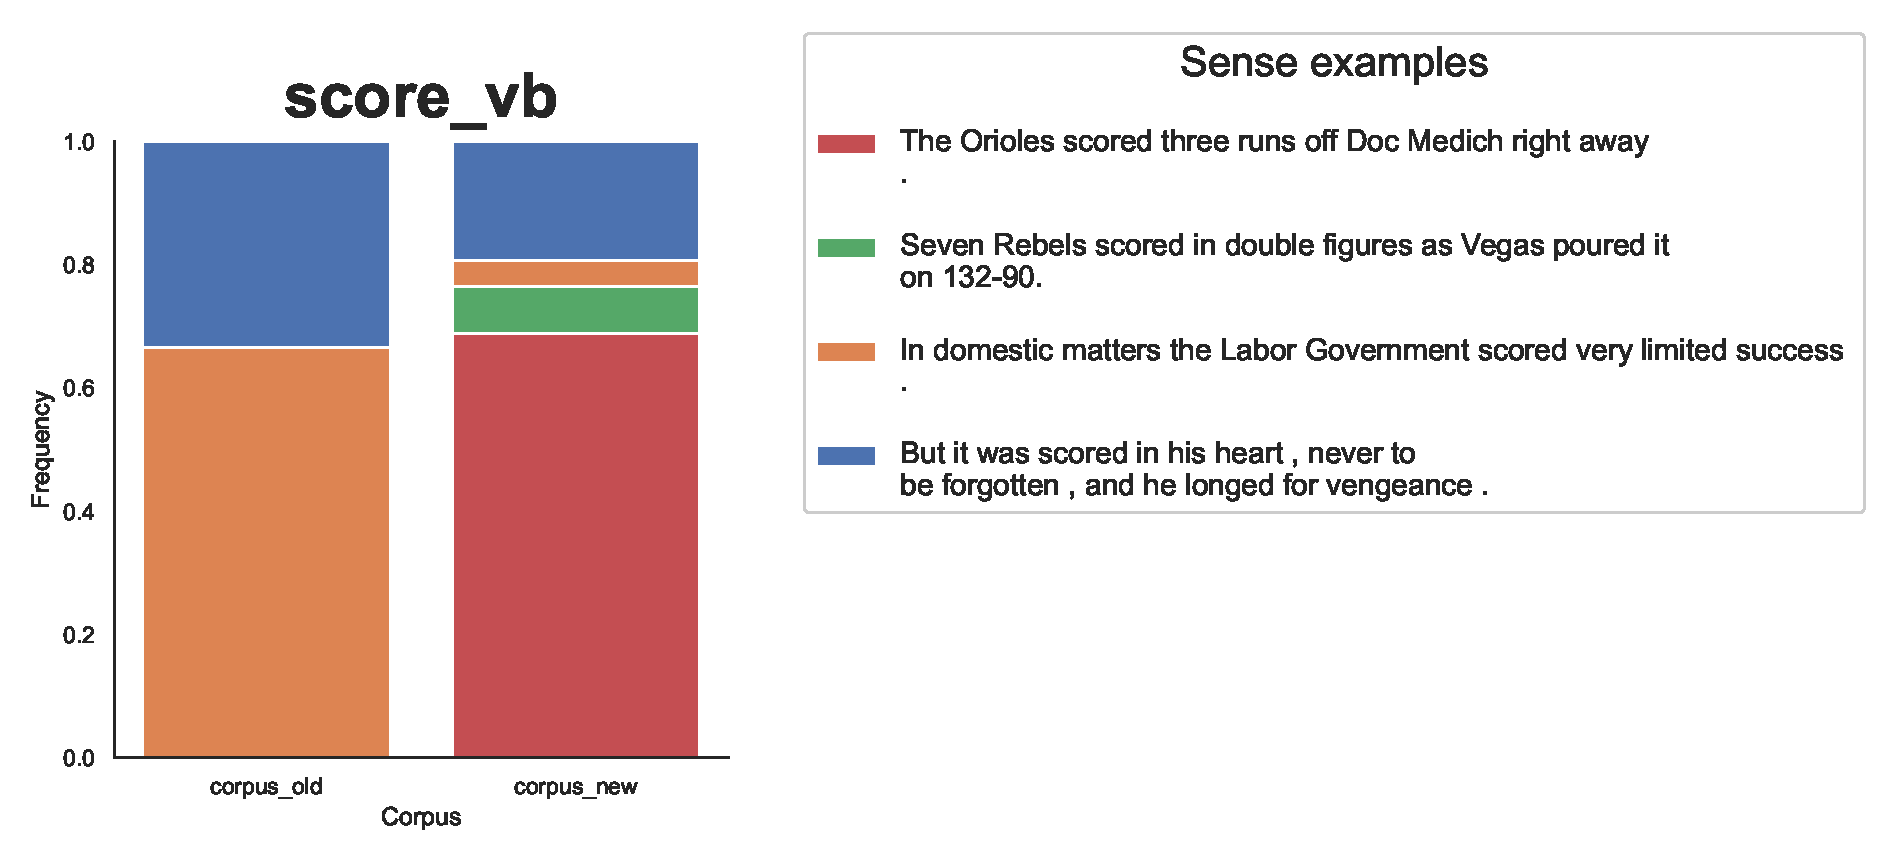
\includegraphics[width=0.7\textwidth]{img/33_score_vb.eps}
    \caption{Shift in the frequency of senses for the verb “score".} 
    \label{fig:semantic_shifts:score}
\end{figure}

The instructions provided for project number 9 stated that the evaluation of the results would be carried out by experts in the linguistics and history domains. To this end, detailed results for each method can be perused in our repository.

Furthermore, we evaluated our results against a ground truth for the semantic shift occurred in 37 words provided by SemEval-2020~\cite{schlechtweg-etal-2020-semeval}. In Table~\ref{tab:semantic_shifts:spearman} we compare the Spearman's rank-order correlation of our methods with the top 5 systems in the SemEval-2020 shared task. We deduce that our methods are competitive with other state-of-the-art systems.

\begin{table}
    \caption{Spearman's rank-order correlation to SemEval-2020 ground truth for the proposed methods and the top systems in the competition.}
    \label{tab:semantic_shifts:spearman}
    \centering
    \begin{tabular}{|c|c|c|c|c|c|c|c|}
        \toprule
        OP & NN & JSD & UG\_Student\_Intern & Jiaxin \& Jinan & cs2020 & UWB & Discovery\_Team \\
        \midrule
        .391 & .341 & .365 & \textbf{.422} & .325 & .375 & .367 & .361 \\
        \bottomrule
    \end{tabular}
\end{table}

\subsection{Conclusion}
\label{subsec:semantic_shifts:conclusion}

Tables~\ref{tab:semantic_shifts:top_words} and~\ref{tab:semantic_shifts:spearman} suggest that, on the LSC task, static embeddings methods perform slightly better than contextualized embeddings methods. The same conclusion can be found in literature~\cite{laicher-etal-2021-explaining,schlechtweg-etal-2020-semeval}. Possible reasons for this behavior are the small size of the corpora for the JSD method and a need of further fine-tuning. Another possible reason lies in the fact that the historical corpus contains a lot of artifacts and wrongly tokenized words.

Apart from these issues, a possible improvement in the JSD method involves tuning the HDBSCAN hyperparameter to find a number of senses for each word that is similar to the number of word synsets found in WordNet.

\section{Historical events extraction}
\label{sec:historical_events}

The second task mentioned in project number 9 involves the detection of historical events in a text and the extraction of the event components, such as dates, historical figures and locations. The Histo Corpus described in~\cite{sprugnoli-tonelli-2019-histo} was suggested for this task. The event recognition model was to be evaluated on Wikipedia pages.

\subsection{Definitions}

The notion of “historical event" is not clearly defined. Since “individuation criteria are not given by nature or language"~\cite{shaw-2010-phdthesis}, ultimately the choice of what constitutes an historical event is arbitrary. In literature, events were labeled as historical when they involved conflicts~\cite{cybulska-vossen-2011-historical}. Here we consider historical such events and entities that may be the subject of a paragraph in a history textbook. These primarily concern military and political occurrences.

\subsection{Data sets}

The Histo Corpus is composed of news and travel narratives from 1865-1926 and is annotated with events, which mainly consist in verbs and participles. Three issues prevented us from using this corpus. 

\begin{enumerate}
    \item The corpus is “historical" in the sense that the documents are not contemporary, but the annotated events are not “historical" in the sense that they are not characterized by historical figures or by episodes that we may find in a history textbook. 
    \item Since the corpus is annotated with “common" events described using a “historical" language, we would have no way to recognize “historical" events described using a “contemporary" language in Wikipedia.
    \item The annotations are limited to the events themselves and do not include event arguments, like dates and people involved in the event.
\end{enumerate}

To the best of our knowledge, there are no public English datasets in which historical events are annotated along with their arguments. An interesting dataset would be the one described in~\cite{lai-etal-2021-event}, in which documents from 1827-1909 are annotated with events related to conflicts and law, along with their arguments. However, this dataset has not yet been disclosed as of the time of this writing.

For the recognition of events and their arguments, we employed the RAMS dataset~\cite{ebner-etal-2020-rams}, in which 139 event types, each with up to 5 arguments, were annotated. Each document of the dataset contains a single event. The peculiarity of this dataset is that the arguments of an event may be found in a different sentence from the one in which the event is mentioned. This makes the task arguably more difficult compared to more well-known datasets, such as ACE 2005\footnote{\url{https://catalog.ldc.upenn.edu/LDC2006T06}}.

We also built a dataset composed of 1024 pages taken from Wikipedia, for a total of approximately 4M tokens. Each page was classified as historical or not based on the properties of the corresponding Wikidata entry. Each page was split into paragraphs to which we assigned the same class of the page, resulting in 16075 historical paragraphs and 23673 non-historical paragraphs. Finally, each paragraph was annotated in the BIO format with the Wikipedia entities mentioned therein, by exploiting the links in the text. Those entities were likewise classified as historical or not based on their Wikidata entry.

\subsection{Strategy}

In tackling the task, we adopted the following strategy. First, we built a model to classify a given paragraph as historical or not. We make the assumption that Wikipedia pages related to historical entities are more likely to describe historical events in their paragraphs. Note that we cannot base our classification solely on the entities mentioned in a paragraph, because: (i) the link to an entity is usually provided only for the first mention and thus only the first mention of an entity can be annotated; (ii) the surface form of an entity can vary greatly (e.g., the text “up the toe of Italy" contains a link to the “Italian campaign (World War II)" entity in the Wikipedia page for Bernard Montgomery).

Once the paragraphs related to historical events were identified, a second model was employed to extract the event and the pertaining arguments.

\subsection{Related work}

In this subsection we briefly outline the models proposed in literature for event and argument extraction. Formally, the problem can be stated as follows. We define an ontology of event types $t \in T$, each of which is associated with a set of $n_t$ arguments $A_t$. Given a document $d = \langle w_1, \dots, w_m \rangle$, we group the $m$ words of the document in $z$ spans $s = \langle w_k, \dots, w_l \rangle \in S$. The problem is then to find which span $s$ (also called “trigger") corresponds to an event $t$, if any, and which spans correspond to the $n_t$ arguments of the event $t$, if any.    

We categorize the models found in literature in two families: span classification approaches and machine reading comprehension (MRC) approaches. We did not consider approaches that exploited external resources, like the Wikipedia and DBpedia ontologies. One such example can be found in~\cite{ahonen-hyvonen-2009-historical}. 

\subsubsection{Span classification approaches} These approaches exploit event and argument annotations to assign labels to each span. There are methods that learn embeddings for each span, possibly adding external features such as POS and dependencies in the parser tree, and then use a neural network~\cite{ebner-etal-2020-rams,zhong-chen-2021-frustratingly,nguyen-nguyen-2019-one-for-all} or transformers~\cite{chen-etal-2020-joint-modeling} to classify each span. Some methods also employ graphs within the process~\cite{lin-etal-2020-oneie,wadden-etal-2019-entity,luan-etal-2019-general,nguyen-2021-gcn}. Most methods extract events and arguments jointly, since pipelining the two tasks is believed to propagate and amplify errors. However, recent approaches are challenging this assumption~\cite{zhong-chen-2021-frustratingly}. 

\subsubsection{MRC approaches} These approaches do not label each span, but rather produce a natural language response to a natural language prompt. These approaches display improved performance in few-shot and zero-shot settings compared to classification approaches. There are models based on slot-filling methods that fill placeholders in a predefined template with spans extracted from the text~\cite{chen-etal-2020-manual,li-etal-2021-genarg}. Other models treat the problem as a question answering task~\cite{du-cardie-2020-event,feng-etal-2020-probing,liu-etal-2020-mrc} or as a textual entailment task~\cite{feng-etal-2020-probing}. Other models yet use sequence-to-structure text generation~\cite{lu-etal-2021-text2event}.

\subsection{Proposed methods}

\subsubsection{Paragraph classification} We adopted a multi-task learning model (MTL) to classify paragraphs as historical or not. First, we obtained BERT embeddings for each token. Then, we used two feed-forward neural networks (FFNN) to jointly learn (i) the paragraph class, and (ii) the tag of the entities referenced in the paragraph. Cross-entropy loss was computed separately for each task and then summed according to learned weights~\cite{kendall-etal-2017-mtl-loss}.

We compared our model with a BiLSTM classifier and a BERT classifier as baseline methods.

\subsubsection{Event and argument extraction} To identify trigger words and thus extract events, we followed the span classification approach described in~\cite{zhong-chen-2021-frustratingly}. After enumerating all spans up to 3 tokens long, we obtained embeddings for each span by aggregating the BERT embeddings of the tokens. Then, we passed the embeddings through a FFNN to classify each span either as an event type $t$ or as a non-event. We used cross-entropy loss.

For argument extraction, we followed the MRC approach described in~\cite{li-etal-2021-genarg,wen-etal-2021-resin}. We fed a BART~\cite{lewis-etal-2020-bart} model with the paragraph and an event template with placeholders “\textlangle{}arg\textrangle{}" for each argument. After training, the model learned to generate the same template with the placeholders filled with text spans. We restricted the language vocabulary to that of the input during generation. We used cross-entropy loss on the logits obtained from the masked language modeling training. 

Event and argument extraction can be performed jointly in a single model by aggregating their losses. We kept the two tasks separated due to hardware constraints and provided the argument model with the gold event type.

We compared our model with results reported in literature.

\subsection{Results}

\begin{table}
    \caption{Accuracy and F1-score of the models for the paragraph classification task.}
    \label{tab:historical_events:classification}
    \centering
    \begin{tabular}{lrr}
        \toprule
        Model & Accuracy & F1-score\\
        \midrule
        MTL & \textbf{0.854} & \textbf{0.716} \\
        BiLSTM & 0.794 & 0.634 \\
        BERT & 0.799 & 0.630 \\
        \bottomrule
    \end{tabular}
\end{table}

\begin{table}
    \caption{Precision (P), recall (R) and F1-score of different models on the official test set of the RAMS data set. TCD stands for type-constrained decoding and refers to the practice of considering only the top-scoring $n_t$ arguments for an event type $t$ with $n_t$ arguments. For our model we reported the micro-average scores.}
    \label{tab:historical_events:event-arguments}
    \centering
    \begin{tabular}{lccccccc}
        \toprule
        & Gold Arg. Spans & \multicolumn{3}{c}{Events} & \multicolumn{3}{c}{Arguments} \\
        Model & & P & R & F1 & P & R & F1\\
        \midrule
        Ebner et al.~\cite{ebner-etal-2020-rams} & Yes & - & - & - & 62.8 & \textbf{74.9} & 68.3 \\
        Ebner et al. (TCD)~\cite{ebner-etal-2020-rams} & Yes & - & - & - & 78.1 & 69.2 & 73.3 \\
        Zhang et al.~\cite{zhang-etal-2020-two} & Yes & - & - & -  & 71.5 & 66.2 & 68.8 \\
        Zhang et al. (TCD)~\cite{zhang-etal-2020-two} & Yes & - & - & -  & 81.1 & 66.2 & 73.0 \\
        Wei et al.~\cite{wei-etal-2021-trigger} & Yes & - & - & - & \textbf{82.0} & 71.6 & \textbf{76.6} \\
        \hline
        Li et al.~\cite{li-etal-2021-genarg} & No & - & - & - & - & - & 48.6 \\
        Zhang et al.~\cite{zhang-etal-2020-two} & No & - & - & -  & - & - & 40.1 \\
        Zhang et al. (TCD)~\cite{zhang-etal-2020-two} & No & - & - & -  & - & - & 41.8 \\
        Wen et al.~\cite{wen-etal-2021-resin} & No & - & - & - & - & - & 48.6 \\
        Wei et al.~\cite{wei-etal-2021-trigger} & No & - & - & - & 53.1 & \textbf{42.7} & 47.4 \\
        Lai et al.~\cite{lai-etal-2021-event} & No & \textbf{71.9} & 74.7 & \textbf{73.2} & - & - & - \\
        Pouran Ben Veyseh et al.~\cite{pouran-ben-veyseh-etal-2021-unleash} & No & 55.5 & \textbf{78.6} & 65.1 & - & - & - \\
        \textbf{Our model} & No & 0.0290 & 0.0287 & 0.0289 & \textbf{62.7} & 42.0 & \textbf{50.3} \\
        \bottomrule
    \end{tabular}
\end{table}

In Table \ref{tab:historical_events:classification} we show the results for the paragraph classification task. Table \ref{tab:historical_events:event-arguments} compares the performances on the event and argument extraction tasks. Note that the authors employed different training settings, such as using gold argument spans and gold event types or considering the syntactical head-words (most representative tokens) of the arguments instead of the whole spans, making it difficult to directly compare the models.

\subsection{Conclusion}

With regard to the paragraph classification task, our MTL model significantly outperforms the baseline methods. The performance could be further improved with a more fine-grained analysis of the Wikidata properties of each Wikipedia page.

Our event model struggles to correctly identify trigger words. One obvious reason is that the vast majority of the spans do not contain events and, therefore, finding not only the correct event span but also the correct event type, from a total of 139 types, becomes a highly imbalanced problem. The results can also be ascribed to the complexity of the data set, whose documents comprise multiple sentences. Moreover, the data set was intended exclusively for argument linking. Finally, trigger words are not limited to verbs, which is at odds with most of the other event detection data sets.

Our argument model compares favourably with the baseline methods. Note that our model does not know the gold argument spans. Indeed, since our model generates text rather than classify spans, it disregards spans altogether.

\bibliographystyle{splncs04}
\bibliography{bibtex_entries}

\end{document}